\documentclass[11pt]{article}
\usepackage{graphicx}
\usepackage{hyperref}
\usepackage[utf8]{inputenc}
\usepackage{amsmath,amsthm,amsfonts,amssymb,amscd}
\usepackage{tikz}
\usepackage{xeCJK}
\usepackage{physics}
\usepackage{multirow,booktabs}
% \usepackage[table]{xcolor}
\usepackage{fullpage}
\usepackage{lastpage}
\usepackage{unicode-math}
\usepackage{enumitem}
\usepackage{fancyhdr}
\usepackage{mathrsfs}
\usepackage{wrapfig}
\usepackage{setspace}
\usepackage{calc}
\usepackage{multicol}
\usepackage{cancel}
\usepackage[retainorgcmds]{IEEEtrantools}
\usepackage[margin=3cm]{geometry}
\usepackage{amsmath}
\DeclareMathAlphabet{\mathcal}{OMS}{cmsy}{m}{n}
\let\mathbb\relax
\DeclareMathAlphabet{\mathbb}{U}{msb}{m}{n}
\newlength{\tabcont}
\setlength{\parindent}{0.0in}
\setlength{\parskip}{0.05in}
\usepackage{empheq}
\usepackage{framed}
\usepackage[most]{tcolorbox}
\usepackage{xcolor}
\linespread{1.2}
\graphicspath{{./}}
\setCJKmainfont[AutoFakeBold = 3, AutoFakeSlant = 4]{BiauKaiTC}
\colorlet{shadecolor}{orange!15}
\parindent 0in
\parskip 12pt
\geometry{margin=1in, headsep=0.25in}
\graphicspath{{./}}
\theoremstyle{definition}
\newtheorem{thr}{Theorem}
\newtheorem{lma}{Lemma}
\newtheorem{defn}{Definition}
\newtheorem{reg}{Rule}
\newtheorem{exer}{Exercise}
\newtheorem{note}{Note}
\newtheorem{asmp}{Assumption}
\begin{document}
\setcounter{section}{0}
\title{Title}

\thispagestyle{empty}
\begin{center}
  {\large \bf HTML HW2} \\ 
  B12901022 廖冠豪
\end{center}
\section*{5}
As the boss of the agent, I disagree with its answer and am greatly disappointed by it. The agent claim that it an first fit the polynomial with the $n - 1$. However $n - 1$ equations isn't enough to specify the $n + 1$ coefficients in the $n$-degree polynomial. Next the agent say that with the polynomial, the $n + 1$-th term of the sequence can be determined This step is correct. The agent then provides an example. In the example, the agent fits the polynomial of degree $2$ with three points. The example is correct because $3$ equations is sufficient for specifying a second degree polynomial. In conclusion, the agent displayed poor mathematical ability by giving positive reply to a mathematically impossible task. It further shows bad logical consistency by trying to prove its false statement with an example that is correct itself but has no significance with respect to the statement.
\newpage
\section*{6}
% We divide the number into four groups
% \begin{gather*}
%   W = {1, 3, 5, 7} \\ 
%   X = {2, 4, 6, 8} \\ 
%   Y = {9, 11, 13, 15} \\ 
%   Z = {10, 12, 14, 16} \\
% \end{gather*}
% We denote the number drawn 
Notice that given any number, the color of it when it is on a A ticket is different to it's color when it is on a B ticket. Similarly, it's color when it is on a C ticket is different to it's color when it is on a D ticket. Therefore, some number on the five tickets to be purely green, that five tickets can't contain A and C tickets at the same time, or B and D tickets at the same time. \\ 
When all the tickets are A or C, all the numbers $9, 11, 13, 15$ are green, and the condition is satisfied. When all the tickets are B or D, all the numbers $2, 4, 6, 8$ are green. When all the tickets are A or D, all the numbers $1, 3, 5, 7$ are green. When all the numbers are B or C, all the numbers $10, 12, 14, 16$ are green. The condition is also satisfied when all the tickets are of the same alphabet.
% From the analysis above, we know that the probability that the condition is met is the probability that all the tickets are A or C plus the probability that all the tickets are B or D. 
Also, since that number of the four kinds of tickets are of the same large quantity, the probability for each drawn ticket to have any specific alphabet is $\frac{1}{4}$.
\begin{gather*}
  P = \underset{AC, AD, BC, BD}{4}\times(\underset{}{(\frac{1}{2})^5} -  2\times\underset{}{(\frac{1}{4})^5}) + \underset{A, B, C, D}{4}\times(\frac{1}{4})^5 \\ 
  = \frac{31}{256}
\end{gather*}
\newpage
\section*{7}
In order that the 5 on a ticket is green, this ticket must be of alphabet A or D. 
\[
  P = (\underset{A}{\frac{1}{4}} + \underset{D}{\frac{1}{4}})^5 = \frac{1}{32}
\]
\newpage
\section*{8}
% \sum_{t^\prime = M + 1}^\infty
We first consider the probability for all $m$ at a fixed $t = t^\prime$.
\begin{gather*}
  P\left(\forall m\in \{1, 2,\dots, M\}\quad \mu_m\leq\frac{c_m}{N_m}+\sqrt{\frac{\ln{t^\prime}+\ln{M} -\frac{1}{2}\ln{\delta}}{N_m}} | t = t^\prime\right) \\ 
  = 1 - P\left((\mu_1 > \frac{c_1}{N_1} + \sqrt{\frac{\ln{t^\prime} + \ln{M} -\frac{1}{2}\ln{\delta}}{N_1}})\cap\dots\cap(\mu_M > \frac{c_M}{N_M} + \sqrt{\frac{\ln{t^\prime} + \ln{M} -\frac{1}{2}\ln{\delta}}{N_M}}) | t = t^\prime\right) \\
  \geq 1 - \sum_{m\in{1, 2,\dots,M}}P\left(\mu_m < \frac{c_m}{N_m} + \sqrt{\frac{\ln{t^\prime} - \frac{1}{2}\ln{\frac{\delta}{M^2}}}{N_m}}\right)
\end{gather*}
Since $0 < \frac{\delta}{M^2} < 1$, we can use the inequality provided in this problem.
\begin{gather*}
  \geq 1 - \sum_{m\in{1, 2,\dots,M}}\frac{\delta}{M^2}t^{-2} = \frac{\delta}{M}t^{-2}
\end{gather*}
Let $A$ denote the event $\forall m \in {1, 2,\dots, M}\quad \mu_m > \frac{c_m}{N_m} + \sqrt{\frac{\ln{t^\prime} + \ln{M} -\frac{1}{2}\ln{\delta}}{N_m}}$, our result in the previous part show that
\begin{gather*}
  P(A | t = t^\prime) \geq 1 - \frac{\delta}{M}t^{-2} \\ 
  \implies P(A^\prime | t = t^\prime) \leq \frac{\delta}{M}t^{-2}
\end{gather*}
\begin{gather*}
  P\left(\forall m\in \{1, 2,\dots, M\}, t \in \{M + 1, M + 2,\dots\} \quad\mu_m\leq\frac{c_m}{N_m}+\sqrt{\frac{\ln{t^\prime}+\ln{M} -\frac{1}{2}\ln{\delta}}{N_m}} \right) \\ 
  = P((A | t = M + 1) \cap (A | t = M + 2) \cap\dots) \\ 
  = 1 - P((A^\prime | t = M + 1) \cap (A^\prime | t = M + 2) \cap\dots) \\
  \geq 1 - \sum_{t^\prime = m + 1}^\infty P(A^\prime | t = t^\prime) \\ 
  \geq 1 - \sum_{t^\prime = m + 1}^\infty \frac{\delta}{M}{t^\prime}^{-2}
  \geq 1 - \frac{\delta}{M} \sum_{t^\prime = 1}^\infty {t^\prime}^{-2} \\ 
  = 1 - \frac{\pi^2\delta}{6M} \\
  \geq 1 - \delta \quad(\frac{\pi^2}{6M} < 1 \quad\text{for}\quad M \geq 2) \\
\end{gather*}
\newpage
\section*{9}
\textbf{The VC bound of the set of symmetric boolean functions is k + 1} \\ 
Proof: \\
First we prove that $d_{VC} \leq k + 1$ \\ 
When there is more than $k + 1$ vectors $\vb{v}\in \{-1, 1\}^k$, pigeonhole principal states that there must exist two vectors $\vb{v}_1, \vb{v}_2$ that has the same number of ones. Since the functions are symmetric, the output they produce given $\vb{v}_1$ and $\vb{v}_2$ must be the same. Therefore, any data set with more than $k + 1$ vectors can't be scattered, and $d_{VC} \leq k + 1$ \\
Next we prove that $d_{VC} \geq k + 1$ \\ 
Consider a data set with $n \geq k + 1$ vectors such that no two vectors have the same number of ones. For any dichotomy, we divide the vectors into two groups, one containing all the vectors with $+1$ as their output, and the other with all the vectors with $-1$. 
  Let $h: \{-1, +1\}^k \rightarrow\{-1, +1\}$ be the boolean function such that for all vectors $\vb{v}$ in this data set $h(\vb{v})$ is equal to its output. Since no two vectors in different groups have the same number of ones, $h$ is symmetric and hence belong to our hypothesis set. Hence the $n$ vectors can be scattered, and $d_{VC} \geq k + 1$. \\ 
  Since $d_{VC} \leq k + 1$ and $d_{VC} \geq k + 1$, we've proven that $d_{VC} = k + 1$.
\newpage
\section*{10}
\begin{gather*}\\
  E_{out} = P[h(x) = +1\cap y = -1] + P[h(x) = -1\cap y = +1] \\ 
  = P[s(x - \theta) > 0 \cap x > 0 \cap y = -1]\\ +  P[s(x - \theta) > 0 \cap x \leq 0 \cap y = -1] \\+  P[s(x - \theta) \leq 0 \cap x > 0 \cap y = +1] \\ +  P[s(x - \theta) \leq 0 \cap x \leq 0 \cap y = +1]
\end{gather*}
We classify the problem into four cases and treat them separately. \\ 
\subsection*{}
$s = +1, \theta\geq0$\\
\begin{gather*}
  E_{out} = \frac{1 - \theta}{2}p + 0 + \frac{\theta}{2}(1 - p) + \frac{p}{2} \\ 
  = p + \frac{\theta}{2} - p\theta
\end{gather*}
\subsection*{}
$s = +1, \theta < 0$ \\ 
\begin{gather*}
  E_{out} = \frac{p}{2} + \frac{-\theta}{2}(1 - p) + 0 + \frac{\theta + 1}{2}p \\ 
  = p - \frac{\theta}{2} + p\theta
\end{gather*}
\subsection*{}
$s = -1, \theta\geq0$\\
\begin{gather*}
  E_{out} = \frac{\theta}{2}p + \frac{1}{2}(1 - p) + \frac{1 - \theta}{2}(1 - p) + 0 \\ 
  = 1 - p + p\theta - \frac{\theta}{2}
\end{gather*}
$s = -1, \theta<0$\\
\begin{gather*}
  E_{out} = 0 + \frac{\theta + 1}{2}(1 - p) + \frac{1}{2}(1 - p) + \frac{-\theta}{2}p \\ 
  = 1 + \frac{\theta}{2} - p\theta - p
\end{gather*}
By the analysis above, we can conclude that for any $h_{s, \theta}$ with $s \in {-1, +1}$ and $\theta \in [-1, 1]$, 
\[
  E_{out}(h_{s, \theta}) = u + v\cdot\abs{\theta}
\]
With 
\begin{gather*}
  u = s(\frac{1}{2} - p) \\ 
  v = \frac{1}{2} - u
\end{gather*}
\newpage
\section*{11}
Scatter plot: \\ 
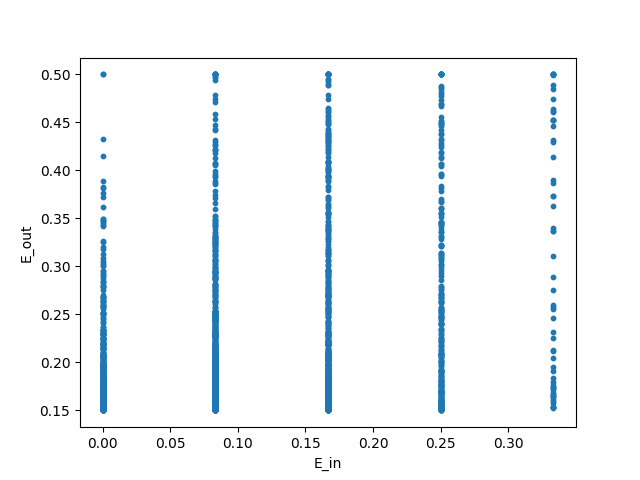
\includegraphics{P11_2.png} \\
\textbf{Median: 1.271091} \\
We see from the scatter plot that all the hypotheses has $E_{out} = 0, 0.08333, 0.166667, 0.25, 0.333333$, which correspond to $0, 1, 2, 3, 4$ errors in the $12$ data points respectively. This means that in the learning processes, no hypothesis that makes more than $4$ error are returned. This is reasonable because the learning algorithm returns the hypothesis with minimal $E_{in}$. \\ 
Code Snapshot: \\ 

\includegraphics[width = \textwidth]{P11code.png}
\newpage
\section*{12}
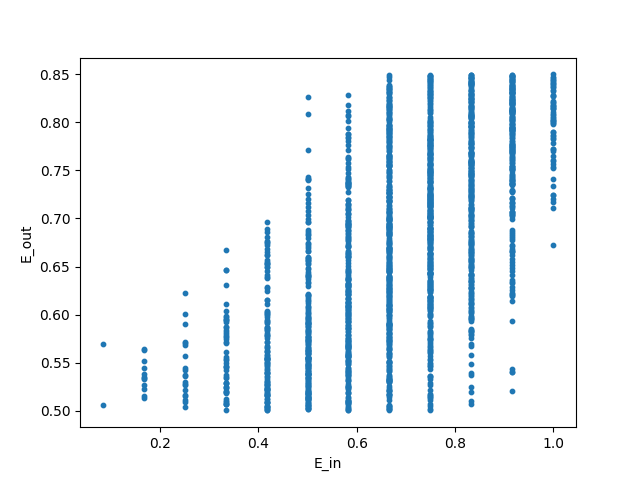
\includegraphics{P12_2.png} \\
\textbf{Median: -0.029372} \\
We see from the scatter plot that in contrast to P11, the number of errors range from $0$ to $12$, this is also reasonable because in this cases we return a random hypothesis instead of an optimal one. We can also see that for larger $E_{out}$ values, the probability for their corresponding $E_{in}$ to be larger is higher. This means that there is a positive relation between $E_{out}$ and $E_{in}$. This is as expected, since Hoeffding's inequality state that the probability of a large difference between $E_{out}$ and $E_{in}$ is upper-bounded. That is to say, $E_{out}$ is close to $E_{in}$ with a considerable probability. \\
Also, we see that the median of $E_{out} - E_{in}$ in P12 is significantly smaller than that in P11. Observe that for hypotheses with a higher number of errors, $E_{in}$ is higher than $E_{out}$ (as can be seen in the case where 12 errors are made and $E_{in}$ is 1 while $E_{out}$ is less than 1), and for hypotheses with a lower number of errors, $E_{in}$ is lower than $E_{in}$ (as can be seen in the case where 0 error is made and $E_{in}$ is 0 while $E_{out}$ is greater than 0). This explains why in P11, where hypotheses with lower $E_{in}$ are chosen, the median of $E_{in} - E_{out}$ is greater than that in P12, where hypotheses are randomly (and uniformly) chosen.  \\
Code Snapshot: \\ 

\includegraphics[width =\textwidth]{P12code.png}
\newpage
\section*{13}
Consider the multi-dimensional positive ray as follows. For data sets that contain $\vb{x} \in \mathbb{R}^d$, we can apply positive ray to one dimension: 
\[
  h^\prime_{i, \theta} = \text{sign}(x_i - \theta)
\]
Let $\mathcal{H}^\prime$ be the hypotheses set that contains all such functions in $\mathbb{R}^d$. \\ 
We represent a dichotomy as $\mathcal{D}_1$, $\mathcal{D}_2$, where $\mathcal{D}_1$ contains all the vectors that are classified as $-1$ and $\mathcal{D}_2$ contains all the vectors that are classified as $+1$.
Consider a dichotomy $\mathcal{D}_1$, $\mathcal{D}_2$ of $n$ data vectors labeled as $\{\vb{x}_1,\dots,\vb{x}_n\}$. This dichotomy can be achieved by $\mathcal{H}^\prime$ if there exist some dimension $i$ such that 
\[
  {v_1}_{i} < {v_2}_{i} \quad \forall \vb{v}_1\in \mathcal{D}_1, \vb{v}_2\in \mathcal{D}_2
\]
Consider the order of the component of the $n$ vectors on dimension $i$, assume that no two vectors have the same component (this is a reasonable assumption to make, as we're trying to separate the data vectors, it's optimal to have vectors that all have different components), this order corresponds to a permutation of $\{\vb{v}_1, \vb{v}_2,\dots,\vb{v}_n\}$. We denote this permutation as $\mathcal{P}$.
From the condition above, we know that the positive ray functions of this dimension $h^\prime_{i, \theta}$ can achieve a dichotomy $\mathcal{D}_1$, $\mathcal{D}_2$ iff for some integer $0 \leq k \leq n$, $\mathcal{D}_1$ is the set of the first $k$ vectors in $\mathcal{P}$. We say that this dichotomy is "dealt with" by the permutation $\mathcal{P}$ if this criteria is met.
Therefore, $\mathcal{H}^\prime$ can scatter $n$ data vectors in $\mathbb{R}^d$ iff there exist $d$ permutations of $\{\vb{v}_1, \vb{v}_2,\dots,\vb{v}_n\}$ and a set of $n$ data vectors such that every dichotomy produced by the data vectors can be dealt with by at least one of the permutations. \\
\bigbreak
Next we consider the following graph.\\
\includegraphics[width = \textwidth]{IMG_101A1D00FD8F-1.jpeg}\\
The graph consists of $n + 1$ layers of nodes, two nodes can only be connected if the difference of their depth is $1$. \\ 
We let each node of depth $k$ represent a subset $k$ of $\{\vb{v}_1, \vb{v}_2,\dots,\vb{v}_n\}$, and two nodes at adjacent depths are connected if one is a subset of another(i.e. you can make the two sets equal by removing one element from the set with larger size). \\ 
% The graph represents many important information in this problem. \\ 
 We can see that at depth $k$ there are ${n\choose k}$ nodes, and one simple path from the top node to the bottom node represents one unique permutation of $\{\vb{v}_1, \vb{v}_2,\dots,\vb{v}_n\}$. \\ 
 By the discussion above, we can also see that we can create a one-to-one relation between a node in the graph to a dichotomy of the $n$ vectors by linking the node with the dichotomy in which all the vectors in the subset represented by the node is classified as $-1$. This way, the nodes in a simple path from top to bottom represents the collection of dichotomies the permutation presented by this simple path can "dealt with". \\
 Hence the scattering problem becomes whether we can find $d$ different simple paths from the top node to the bottom node such that all node is visited at least once by a path. \\
 \medbreak
 We then prove that for scatter to happen, we must have $d \geq {n\choose \lfloor\frac{n}{2}\rfloor}$. \\
 Proof: \\
 We notice that the depth at which there are the most nodes is $k = \lfloor\frac{n}{2}\rfloor$, with ${n\choose \lfloor\frac{n}{2}\rfloor}$ nodes. If $d < {n\choose \lfloor\frac{n}{2}\rfloor}$ clearly there must be unvisited node(s) at depth $\lfloor\frac{n}{2}\rfloor$, so scattering is not possible. \\ 
 % \begin{lma}
 %   Consider the two layers of the graph of depth $k$ and $k + 1$ respectively. Let $n_k$ and $n_{k + 1}$ be the number of nodes at the two layers. WLOG, assume that$n_k \geq n_{k + 1}$. Then there exists a set of $n_k$ edges between nodes of the two layers such that every node at depth $k$ connects with exactly one edge, and every node at depth $k + 1$ connects with at least one edge. \\ 
 %   Proof: \\ 
 %   We know that for each node at depth $k$, it is connected with $n - k$ edges that go downwards to depth $k + 1$. For each node at depth $k + 1$, it is connected with $k + 1$ edges that go upwards to depth $k$. \\
 %   % Suppose that we have successfully connected the first $m$ nodes at depth $k + 1$ with $m$ different nodes at depth $k$.
 %   Notice that we can always link the $n_{k + 1}$ nodes at depth $k + 1$ to $n_{k + 1}$ different nodes at depth $k$. This is because 
 %
 % \end{lma}
 % Next, starting from the ${n\choose \lfloor\frac{n}{2}\rfloor}$ nodes at depth $k$, we prove that there exist $d$ simple paths starting from depth $k$ ending at depth $n$ that visits all the nodes of depth no smaller than $k$ at least once. Consider depth $k + 1$. Since the nodes at this depth is less than or equal to the number of nodes at depth $k$, by symmetric arguments we can see that we can also visit all the nodes at depth $k + 1$ (the symmetry here is that the number of edges that starts from a node at depth $k$ and ends at a node at depth $k + 1$ is the same for all nodes at depth $k$, and is also same for all nodes at depth $k + 1$, this symmetry means that the paths starting at depth $k$ can visit the nodes at $k + 1$ equally, and since there are no less paths than nodes, every node is visited). By induction, we can further prove that all nodes below depth $k$ can be visited. Similarly, starting at depth $k$, all nodes above depth $k$ can also be visited. Since the graph is not directed, we can combine a path that starts from some node at depth $k$ and ends at the bottom node and another path that starts from the same node at depth $k$ and ends at the top node into a path from the top node to the bottom node. \\ 
 % We have thereby proven that $d = {n\choose \lfloor\frac{n}{2}\rfloor}$ is the smallest possible dimension to scatter a data set of vectors of size $n$. \\ 
 Hence the VC dimension of $\mathcal{H}^\prime$ is upper-bounded by
 \[
   d^\prime_{VC} \leq \tilde{d}
  % {n\choose \lfloor\frac{n}{2}\rfloor} \leq d
 \]
 Where $\tilde{d}$ is the largest integer such that
 \[
   {\tilde{d}\choose \lfloor\frac{\tilde{d}}{2}\rfloor} \leq d
 \]
 \medbreak
 For the last part of this problem, we prove that the VC dimension of $\mathcal{H}^\prime$ and the VC dimension of $\mathcal{H}^\prime$ is related by $d_{VC}^\prime + 1= d_{VC}$ \\ 
 \medbreak
 First we prove that $d^\prime_{VC} + 1 \leq d_{VC}$ \\ 
 Suppose that $\mathcal{H}^\prime$ can scatter $n$ data vectors $\{\vb{v}_1, \vb{v}_2,\dots,\vb{v}_n\}$, that is, it can produce all $2^n$ dichotomies. Now consider using the decision stump model instead of the positive ray model. (That is, for every $h^\prime_{i, \theta}$ positive ray function that is previously used, we now use $h_{-1, i, \theta}$ and $h_{+1, i, \theta}$ to classify the set of vectors) In this case all the dichotomies are produced twice. We now insert a new data vector $\vb{v}^\prime$ to the set of $n$ vectors. We choose $\vb{v}^\prime$ such that
 \[
   \vb{v}^\prime_i > \vb{v}_i\quad \forall \vb{v}\in \{\vb{v}_1, \vb{v}_2,\dots,\vb{v}_n\}, \quad i \in \{1, 2,\dots,d\}
 \]
 And
 \[
   \vb{v}^\prime_i > \theta \quad \forall \theta \in \mathcal{T}_i
 \]
 Where $\mathcal{T}_i$ is the set containing all the $\theta$ factors used for the positive ray model on dimension $i$ to produce the dichotomies. \\ 
 This way, if $h_{+1, i, \theta}$ and $h_{-1, i, \theta}$ produce the same dichotomy for $\{\vb{v}_1, \vb{v}_2,\dots,\vb{v}_n\}$, they produce two different dichotomies for $\{\vb{v}_1, \vb{v}_2,\dots,\vb{v}_n, \vb{v}^\prime\}$ \\ 
 Therefore, we see that if $\mathcal{H}^\prime$ can scatter $n$ data vectors, $\mathcal{H}$ can scatter $n + 1$ data vectors. \\ 
 \medbreak
 Next we prove that $d^\prime_{VC} + 1 \geq d_{VC}$ \\ 
 Suppose that $\mathcal{H}$ can scatter $n + 1$ data vectors $\{\vb{v}_1, \vb{v}_2,\dots,\vb{v}_n, \vb{v}^\prime\}$. We first adjust the order of these $n + 1$ vectors on each dimension such that $\vb{v}^\prime$ is always classified as $+1$ by a hypothesis $h$ with $s = +1$. (If $\vb{v}^\prime$ is classified as $-1$ on some dimension, we just reverse the order of all the vectors' components of that dimension, then by symmetry between $h_{-1, i, \theta}$ and $_{+1, i, \theta}$, we see that set of vectors is stilled scattered by the same set of decision stump functions.) Now consider using the positive ray model instead of the decision stump model. (That is, for every pair of $h_{-1, i, \theta}$ and $h_{+1, i, \theta}$, that is previously used, we now use $h^\prime_{i, \theta}$ to classify the vectors) We see that of the $2^{n + 1}$ dichotomies we previously had, only the ones where $\vb{v}^\prime$ is classified as $+1$ is left. Now we remove $\vb{v}^\prime$ from the set of vectors, and we are left with the $2^n$ dichotomies of the $n$ vectors in $\{\vb{v}_1, \vb{v}_2,\dots,\vb{v}_n\}$. Hence we've proven that if $\mathcal{H}$ can scatter $n + 1$ data vectors, $\mathcal{H}^\prime$ can scatter $n$ data vectors. \\ 
 Therefore $d^\prime_{VC} + 1 \geq d_{VC}$
 We now have $d^\prime_{VC} + 1 = d_{VC}$ \\
 Hence the VC dimension of $\mathcal{H}^\prime$ 
 \[
   d_{VC} = \tilde{d} + 1
 \]
 Where $\tilde{d}$ is the largest integer such that 
 \[
   {\tilde{d}\choose \lfloor\frac{\tilde{d}}{2}\rfloor} \leq d
 \]
 \bigbreak
 On a further note, by the argument of the graph and simple paths made above, we can see that if we have $d \geq {n\choose \lfloor\frac{n}{2}\rfloor}$ we can have $d$ simple paths from the top node to the bottom node that visit every node at least once. Therefore, the $\tilde{d} + 1$ we obtained above is also a lower bound for $d_{VC}$, and $\tilde{d} + 1$ not only bounds, but is also the precise value of $d_{VC}$
% \textbf{This problem is done in collaboration with B12901035 鄭宇彥}
% Let $\mathcal{H}_{i^\prime}$ be the subset of $\mathcal{H}$ that contains all hypotheses $h_{s, i, \theta}$ of one specific dimension $i = i^\prime$. Clearly this set of hypotheses can only produce $2n$ dichotomies, as the 1D case of this problem is simply the positive ray. Therefore, with $2^n$ dichotomies and $d$ dimensions in total we achieve a bound for $n$ such that the data vectors can be scattered.
% \[
%   2nd \geq 2^n
% \]
% We then apply this bound to $d_{VC}$ \\ 
% \begin{align*}
%   2d_{VC}d \geq 2^{d_{}} \\ 
%   \implies d_{VC} &\leq \lg(2d_{VC}d) = 1 + \lg{d} + \lg{d_{VC}}  \\
%   &\leq 1 + \lg{d} + \lg(1 + \lg{d} + \lg{d_{VC}})
% \end{align*}
\end{document}
